If data stayed amongst those that owned or governed it, then there would be less of a need for privacy preserving mechanisms. 
However in FL, while clients do process data on their own devices, the results are then sent to a centralised server for aggregation. 
\\ \\
In FL we are trying to have all the clients keep hold of their data whilst still being able to contribute it in a form that does not actually involve the sharing of it. The data is usually uneven as each client involved could have wildly different sizes of data or even wildly different backgrounds for the data. Two examples of this would be:
\begin{enumerate}
    \item Monitoring users' interactions with an app and training a model on the user's phone to make accurate predictions about what ads they'll like. 
    The model update calculated will be hyper-specific and over-fitted to an individual user at first. 
    But when you get 10s of 100s of users' models all being sent to a centralised server for aggregation, the model that will be sent back to each user will be much more generalised and better at making more accurate/clever predictions. 
    Through more rounds of back and forth it will eventually converge.
    
    \item If you had a group of hospitals that all had a large amount of patient data and they wanted to train a model for some arbitrary reason, they would be able to again train locally and send off the model just like before. 
    However, you could end up having 1 hospital that deals with a disproportionately large amount of elderly patients and their model would be skewed in that favour. 
    This can help the other hospitals who do not have as much access to such data. 
    This is a mutually beneficial exchange, as it also gives the original hospital more access to younger patient data. 
    As such, results are more easily able to generalise regardless of the age.
\end{enumerate}
As you can see, through FL, we are able to get more accurately trained models on otherwise private and sensitive data. 
This provides unprecedented potential for medical data to be used for research purposes where we will not need direct access to the data. However, as too-good-to-be-true as this might sound, there are obvious barriers in the way. 
For the hospitals and practices, not only will they have to standardise all of their data in an agreed-upon way, they will also have to hugely invest in some form of computing infrastructure such as something on-premise or in the cloud \cite{future_health_fl}. 
This involves a high initial cost as there is computing power needed for training such large amounts of data. 
This also does not mean that researchers outside of the hospital will even be able to use the data anyway, just that the Clinicians, Patients, Manufacturers and Healthcare providers can all benefit from the improvement of the ML-based systems \cite{future_health_fl}.

\subsection{Training}
The process of training the data for Fl is as follows and is shown graphically in Figure \ref{fig:federated_learning}:
\begin{enumerate}
    \item Clients retrieve model from the central server.
    
    \item Each Client trains the model on its data and calculates a model update.
    
    \item Clients send the updates to the central server.
    
    \item Central server aggregates these updates together.
    
    \item Central server sends the new shared model back to the clients.
    
    \item Repeat 1-5 until convergence.
\end{enumerate}
\begin{figure}[htbp]
	\centering
    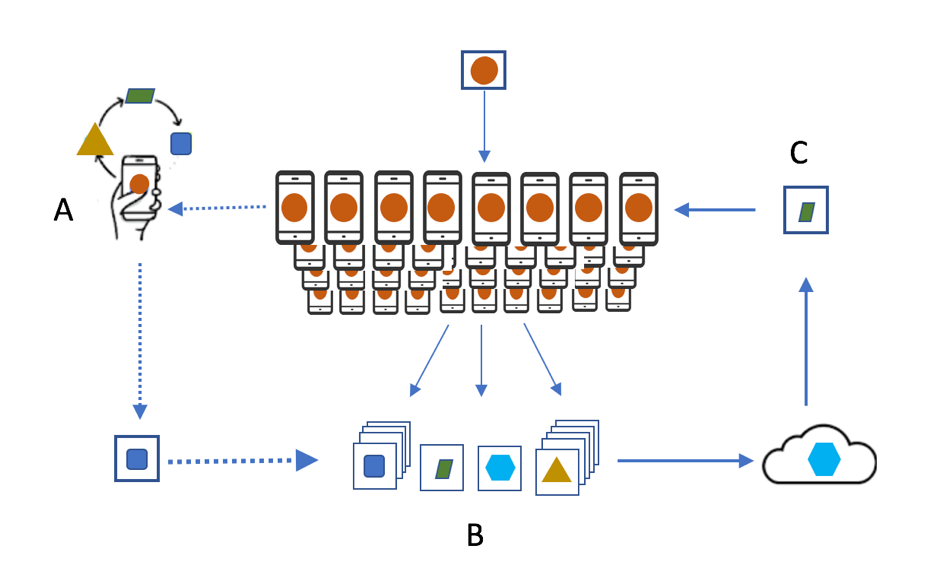
\includegraphics[scale=0.3]{background/federated_learning.png}
	\caption{Rough example of the exchange of ML models on user devices \cite{federated_learning}}
	\label{fig:federated_learning}
\end{figure}
The process by which the aggregation could be done is usually one of Federated Stochastic Gradient Descent (FedSGD) \cite{fedsgd} or Federated Averaging (FedAvg) \cite{fedavg}.
FedSGD aggregates on the models' gradients whereas FedAvg aggregates on the models' weights/parameters. \\ \\
In comparison to a baseline model with no FL employed, close to the exact same results can be achieved with standard FL with between a 0.008 and 0.014 Area under the Curve (AUC) difference \cite{babu}.


\subsection{Personalised Federated Learning}
Through this typical process of training, every client receives the same global model that has been aggregated through a contribution from everyone in some way, shape or form.
However, this might end up not being the most ideal strategy for achieving the best accuracy globally and locally.
Especially when it comes to non-independent and identically distributed (iid) data, being able to adapt the models that are sent out could be crucial for getting good performance.
\\ \\
One style in which this can be done is with Federated First Order Model Optimisation (FedFomo) \cite{fedfomo}.
Here, the method involves each client having a goal that it aims for that is based on its own validation and test data.
The central server then tries to group clients that want to achieve similar goals together so that they can contribute towards their own model together.
\\ \\
This method is a tad odd in that it does not seem to focus on generalisation and making sure the models utilise all of the data from the clients in a constructive way.
However, there are a variety of different ways in which this personalisation could be implemented and ultimately the solution chosen should reflect the problem that is trying to be solved.


\subsection{Privacy Amplification}
Attempting to amplify privacy via user sampling is a method in which not all clients are chosen to participate at every federated round.
Its main use is for helping to preserve the privacy of the clients involved through minimising honest-but-curious clients' interest in information leakage.
\\ \\
This seems like it would be an interesting solution to help the clients' privacy but unfortunately it is not without its drawbacks.
Experiments have shown that generally decreasing the probability (p) for clients to be picked leads to quite a significant decrease in convergence rate as well as a decrease in training accuracy \cite{privamp}.
\\ \\
Depending on what trade-offs you are willing to make, its gives the user quite a bit of flexibility in terms of having either more privacy, better accuracy or some combination of both.



\subsection{Possible Attacks}
Aggregating on the model updates from distributed clients seems to be a great strategy for accessing private data without it being leaked out. 
However, as all things that involve a human element, it can be exploited. 
The two main types of attacks are targeted and untargeted attacks.
Targeted attacks focus on the attacker trying to get the model to predict a specific thing incorrectly, e.g. telling an MNIST dataset that 5 is actually 7 to the extent that the global model starts classifying it as such. 
Untargeted attacks are just when the attacker tries to get the model to not reach convergence or a good accuracy.
\\ \\
Some different styles of poisoning (changing something in a negative manner) are highlighted in Table \ref{tbl:poisoning}. 
All methods excluding the final option are easily accessible to any client.
This is because the client owns their data and as such is in full control and can change it as needed. 
In terms of model reading and writing, the client will receive the model and can send back whatever they like. 
The central server has no way of stopping any of this and without breaking the whole notion behind federated learning, cannot have the clients data checked for tampering (unless some encrypted form of ML was used, which is extremely slow and computationally expensive). \\ \\
In theory if you had control of the client side as well (e.g. a mobile app), then you probably would not need to worry about the model poisoning side of things. 
The final option assumes that the malicious client essentially has complete control over the system and at this point it is essentially impossible to design a robust aggregation system \cite{robagg_fl}.
\begin{center}
    \begin{longtable}{ |c|c|c|c|c| }
    \caption{Poisoning Attacks \& Corruption Examples \cite{robagg_fl} - \textbf{Data Write} is changing of data in dataset, \textbf{Model Read} executing code based on model update before update takes place, \textbf{Model Write} is running code instead of standard update code and \textbf{Aggregation} is running code instead of the standard aggregation function on the central server}
    \label{tbl:poisoning}
    \hline
    \textbf{Corruption Type} & \textbf{Data Write} & \textbf{Model Read} & \textbf{Model Write} & \textbf{Aggregation} \ \\ \hline
    None & - & - & - & - \ \\ \hline
    Static Data Poisoning & Yes & - & - & - \ \\ \hline
    Adaptive Data Poisoning & Yes & Yes & - & - \ \\ \hline
    Update Poisoning & Yes & Yes & Yes & - \ \\ \hline
    Byzantine & Yes & Yes & Yes & Yes \ \\ \hline
    \end{longtable}
\end{center}
There's also the case to handle where it may look like an attacker is trying to cause damage when it actuality it's just a faulty client. 
Depending on the level of damage done it may be beneficial to actually not block faulty clients, as they may introduce noise that improves the model's generalisability \cite{dnn_noise, robust_corrupt_noise}. 
However, you are most likely going to end up blocking them as they could be damaging your performance without themselves realising it.

\subsubsection{Data Poisoning}
This involves maliciously changing the data in an attack. 
It could be done by adding noise or changing labels but as long as the original dataset has been changed, it is considered as having undergone a data poisoning attack. 
It has been shown that data poisoning attacks have been able to achieve a high-confidence of misclassification for deep NN \cite{poison_dnn}. 
\\ \\
There is also a difference between static and adaptive data poisoning. 
Static is where the data is poisoned once at the beginning (prior to training). 
Adaptive is seeing how the models change and then change the data at the beginning of each round so as to accommodate for it. 
Adaptive is more complex but could have the potential to achieve better results as the attack ends up being more tailored.

\subsubsection{Model Poisoning}
This technique uses the model to help craft a specially designed model update. 
In the targeted case, we would have a goal for misclassification but with all of the other users averaging out the poisoning, we would need to change the update in such a way as to negate the combined effects of the benign clients.
Evaluation done has shown that this can lead to 100\% confidence in target misclassification while also impressively achieving convergence of the model \cite{adversarial_lens}. 
\\ \\
To help avoid detection (if the aggregation done is attempting to be robust) where the central server has stealth metrics to identify malicious clients, the malicious objective can be modified so as to account for these detections. 
With this you can normally go undetected for the majority of the rounds but a more clever strategy where we use ``alternating minimisation" to account for both stealth and model poisoning so as to help go undetected for all of the rounds \cite{adversarial_lens}. 
The aim is to minimise for the adversarial objective first and then minimise for the stealth objective for any given epoch.

\subsubsection{Free-Riding}
Attacks do not necessarily come in the form of trying to manipulate the model in a negative way. 
One method involves ``Free-Riding" \cite{free_riding} where the client instead has a goal of trying to gain the completed model without actually contributing anything to the cumulative effort. 
This might be done when the models have commercial/intellectual value and can subsequently lead to intellectual property/financial loss. 
The client would have to trick the rest of the clients into thinking that they have useful and valuable data to contribute.
The size at which the free-rider decides to claim their data is up to them, but is typically the average of the rest of the data.
\\ \\
The initial way of doing this would be to simply return the model's parameters at each round. 
However, this can easily be checked for by the central server.
The way to get around this is to add some Gaussian white noise to the parameters and gradients that is of a similar structure to the benign clients' responses.
This is done by monitoring the mean and variance of the other responses and adjusting accordingly at each round.
The main effect adding noise has is that the resulting variance of the accuracy will increase and the amount it increases is dependant on the variance used by the free-rider.
However, it should be noted that the increase in variance did not appear to show a significant increase in loss and so it could be considered worth it for the anonymity.
\\ \\
However, the noise variation that is typically observed by the benign clients, through something like SGD, decreases as the model converges.
So the free-rider must in turn decrease their noise in a similar asymptotic manner to their noise added.
This again works until a certain extent but anomaly detection methods such as Deep Autoencoding Gaussian Mixture Models (DAGMM) \cite{dagmm} have been shown to detect the free-riders as anomalies \cite{freerider_defence}.
\\ \\
The main way for free-riding clients to then hide is to use a ``delta-weight attack" \cite{freerider_defence}.
Here, they instead use the difference between the previous and current global models and assign that difference to the gradient weights of the parameters.
This emulates the average gradient weights from all of the other clients and so becomes a very neutral client and so can avoid detection much better.
Wonderfully, with the use of privacy amplification, it becomes easier for the central server to detect these delta-weight attacks.
This is because they are only getting model updates every few rounds when selected and so their model that they contribute has gradients with far more eccentric changes than they would otherwise have.
\\ \\
``This result is in agreement with our theory, for which the convergence speed is inversely proportional to the relative size of the free-riders" \cite{free_riding}. 
However, it should be noted that too many free-riders will detriment the global model to some extent and so these attackers should be wary of the effect that they have.
This becomes slightly less of a problem with DP as the inherent added noise almost mimics that of a free-rider and so there is more expectation of fluctuations of accuracy.
It also allows the free-riders to hide themselves better amongst the other clients, which is a nice added bonus for them.
\\ \\
The nature of free-riding becomes quite an elusive game of cat-and-mouse with ever increasing concealing and detection.
It's quite a wondrous area for further investigation and implementation testing.


